\section{Oracle附加说明文档}

数据持久化是确保数据库在服务器因故障重启或数据库重新挂载时不会丢失数据的重要措施。本数据库在Ubuntu服务器上通过Docker实现了数据持久化,从而保证了数据的可靠性和持久性。

\subsection{部署阿里云轻量应用服务器}

轻量应用服务器(Simple Application Server),是可快速搭建且易于管理的轻量级云服务器;提供基于单台服务器的应用部署,安全管理,运维监控等服务,一站式提升您的服务器使用体验和效率。服务器版本信息见\cref{fig:ServerVersion},服务器防火墙规则见{tab:FirewallRules}。

服务器配置详情:

\begin{itemize}
	\item \textbf{实例ID}:dfc3f736506748c3ba9ced56b94a81d7
	\item \textbf{实例名称}:轻量应用服务器
	\item \textbf{地域}:中国香港
	\item \textbf{配置信息}:2核 vCPU | 4GB 内存 | 3072GB 每月流量 | 80GB ESSD | 30Mbps 限峰值带宽
	\item \textbf{镜像信息}:Ubuntu 22.04
	\item \textbf{私有IP地址}:172.19.54.72
	\item \textbf{公有IP地址}:47.238.195.140
	\item \textbf{到期时间}:2024年10月8日 00:00:00
	\item \textbf{配置费用}:¥102.00(优惠金额¥300.00)
\end{itemize}

\begin{figure}[htbp]
	\centering
	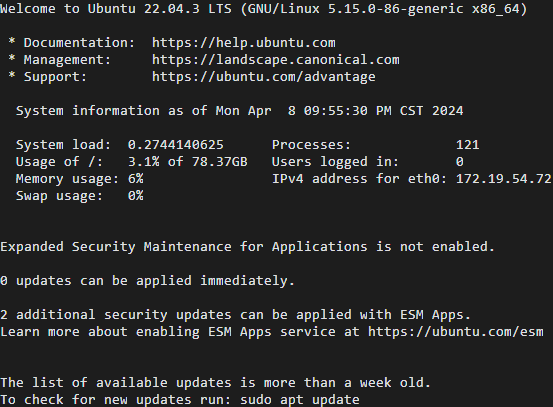
\includegraphics[width=0.8\textwidth]{figures/ServerVersion.png}
	\caption{服务器版本信息}
	\label{fig:ServerVersion}
\end{figure}

\begin{longtable}[c]{@{}lrll@{}}
	\caption{防火墙规则}
	\label{tab:FirewallRules}                                                 \\
	\toprule
	\textbf{协议} & \textbf{端口范围} & \textbf{限制IP来源} & \textbf{备注}               \\ \midrule
	\endfirsthead
	\multicolumn{4}{r}{\textbf{续表~\thetable}}                                 \\
	\toprule
	\textbf{协议} & \textbf{端口范围} & \textbf{限制IP来源} & \textbf{备注}               \\ \midrule
	\endhead
	\hline
	\multicolumn{4}{r}{续下页}
	\endfoot
	\endlastfoot
	TCP         & 80            & 0.0.0.0/0       & HTTP 默认端口                 \\
	TCP         & 443           & 0.0.0.0/0       & HTTPS 默认端口                \\
	TCP         & 1521          & 0.0.0.0/0       & PetJoy Oracle Database 端口 \\
	TCP         & 5101          & 0.0.0.0/0       & PetJoy DatabaseWebAPI 端口  \\
	TCP         & 22            & 0.0.0.0/0       & SSH 远程服务默认端口              \\ \bottomrule
\end{longtable}

\subsection{部署Docker环境}

部署Docker环境的流程如下:

\begin{enumerate}
	\item 设置Docker的apt仓库
	\begin{minted}[baselinestretch=1]{bash}
		# Add Docker's official GPG key:
		sudo apt-get update
		sudo apt-get install ca-certificates curl
		sudo install -m 0755 -d /etc/apt/keyrings
		sudo curl -fsSL https://download.docker.com/linux/ubuntu/gpg -o /etc/apt/keyrings/docker.asc
		sudo chmod a+r /etc/apt/keyrings/docker.asc
		
		# Add the repository to Apt sources:
		echo \
		"deb [arch=$(dpkg --print-architecture) signed-by=/etc/apt/keyrings/docker.asc] https://download.docker.com/linux/ubuntu \
		$(. /etc/os-release && echo "$VERSION_CODENAME") stable" | \
		sudo tee /etc/apt/sources.list.d/docker.list > /dev/null
		sudo apt-get update
	\end{minted}
	\item 安装Docker
	\begin{minted}[baselinestretch=1]{bash}
		sudo apt-get install docker-ce docker-ce-cli containerd.io docker-buildx-plugin docker-compose-plugin
	\end{minted}
	\item 查看Docker版本,验证Docker安装是否成功(\cref{fig:ClientDockerVersion}、\cref{fig:ServerDockerVersion})
	\begin{minted}[baselinestretch=1]{bash}
		docker version
	\end{minted}
\end{enumerate}

\begin{figure}[htbp]
	\centering
	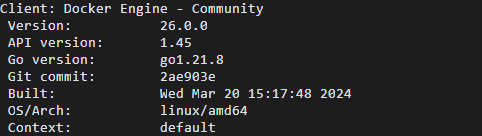
\includegraphics[width=0.8\textwidth]{figures/ClientDockerVersion.png}
	\caption{客户端Docker版本信息}
	\label{fig:ClientDockerVersion}
\end{figure}

\begin{figure}[htbp]
	\centering
	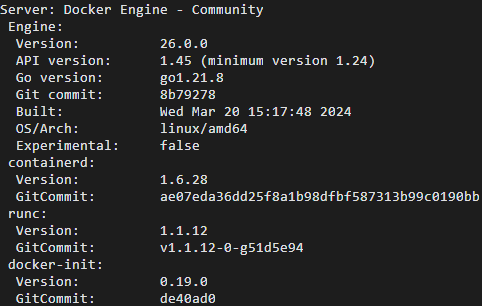
\includegraphics[width=0.8\textwidth]{figures/ServerDockerVersion.png}
	\caption{服务端Docker版本信息}
	\label{fig:ServerDockerVersion}
\end{figure}

\subsection{数据持久化方式部署Oracle 12c数据库}

数据持久化方式部署Oracle 12c数据库的流程如下:

\begin{enumerate}
	\item 下载镜像文件
	\begin{minted}[baselinestretch=1]{bash}
		docker pull absolutapps/oracle-12c-ee:latest
	\end{minted}
	\item 查看镜像文件
	\begin{minted}[baselinestretch=1]{bash}
		docker images
	\end{minted}
	\item 创建主机内路径
	\begin{minted}[baselinestretch=1]{bash}
		mkdir -p /home/local/oracle-data
	\end{minted}
	\item 在 Docker 容器内运行 Oracle 12c 数据库
	\begin{minted}[baselinestretch=1]{bash}
		docker run -d --name petjoy-oracle-database --privileged -v /home/local/oracle-data:/u01/app/oracle -p 8080:8080 -p 1521:1521 absolutapps/oracle-12c-ee
	\end{minted}
	\item 查看容器启动日志(\cref{fig:ContainerStartupLog})
	\begin{minted}[baselinestretch=1]{bash}
		docker logs -f petjoy-oracle-database
	\end{minted}
	\item 查看容器状态
	\begin{minted}[baselinestretch=1]{bash}
		docker ps
	\end{minted}
\end{enumerate}

\begin{figure}[htbp]
	\centering
	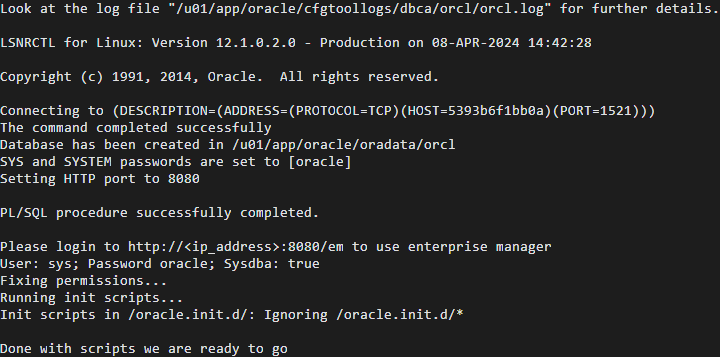
\includegraphics[width=0.8\textwidth]{figures/ContainerStartupLog.png}
	\caption{容器启动日志}
	\label{fig:ContainerStartupLog}
\end{figure}

\subsection{测试Oracle 12c数据库}

测试Oracle 12c数据库的流程如下:

\begin{enumerate}
	\item 进入容器
	\begin{minted}[baselinestretch=1]{bash}
		docker exec -it petjoy-oracle-database /bin/bash
	\end{minted}
	\item 切换数据库用户
	\begin{minted}[baselinestretch=1]{bash}
		su oracle
	\end{minted}
	\item 进入数据库(\cref{fig:AccessToDatabase})
	\begin{minted}[baselinestretch=1]{bash}
		$ORACLE_HOME/bin/sqlplus / as sysdba
	\end{minted}
	\item 查询数据库状态
	\begin{minted}[baselinestretch=1]{sql}
		select status from v$instance;
	\end{minted}
\end{enumerate}

\begin{figure}[htbp]
	\centering
	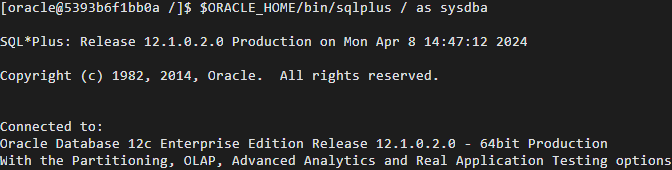
\includegraphics[width=0.8\textwidth]{figures/AccessToDatabase.png}
	\caption{进入数据库}
	\label{fig:AccessToDatabase}
\end{figure}

\subsection{添加Oracle 12c数据库用户}

添加Oracle 12c数据库用户的流程如下:

\begin{enumerate}
	\item 连接到数据库作为 SYSDBA
	\begin{minted}[baselinestretch=1]{sql}
		conn system/oracle as sysdba;
	\end{minted}
	\item 修改 system 用户的密码为 oracle
	\begin{minted}[baselinestretch=1]{sql}
		alter user system identified by oracle;
	\end{minted}
	\item 修改 sys 用户的密码为 sys
	\begin{minted}[baselinestretch=1]{sql}
		alter user sys identified by sys;
	\end{minted}
	\item 修改默认的密码策略,将密码的有效期限设置为无限
	\begin{minted}[baselinestretch=1]{sql}
		ALTER PROFILE DEFAULT LIMIT PASSWORD_LIFE_TIME UNLIMITED;
	\end{minted}
	\item 创建一个新用户 tjsse\_dbteam,并且设置其密码为 tjsse2024
	\begin{minted}[baselinestretch=1]{sql}
		create user tjsse_dbteam identified by tjsse2024;
	\end{minted}
	\item 为 tjsse\_dbteam 用户授权
	\begin{minted}[baselinestretch=1]{sql}
		grant connect, resource, dba to tjsse_dbteam;
	\end{minted}
	\item 查询数据库账户
	\begin{minted}[baselinestretch=1]{sql}
		SELECT username FROM dba_users;
	\end{minted}
\end{enumerate}

\subsection{以tjsse\_dbteam用户身份连接数据库}

可以通过轻量应用服务器和JetBrains DataGrip以tjsse\_dbteam用户身份连接数据库。

\subsubsection{通过轻量应用服务器连接数据库}

通过轻量应用服务器连接数据库的流程如下:

\begin{enumerate}
	\item 进入容器
	\begin{minted}[baselinestretch=1]{bash}
		docker exec -it petjoy-oracle-database /bin/bash
	\end{minted}
	\item 切换数据库用户
	\begin{minted}[baselinestretch=1]{bash}
		su oracle
	\end{minted}
	\item 进入数据库
	\begin{minted}[baselinestretch=1]{bash}
		$ORACLE_HOME/bin/sqlplus
	\end{minted}
	\item 输入用户名和密码
\end{enumerate}

\subsubsection{通过JetBrains DataGrip连接数据库}

通过JetBrains DataGrip连接数据库(\cref{fig:ConnectViaDataGrip}):

\begin{figure}[htbp]
	\centering
	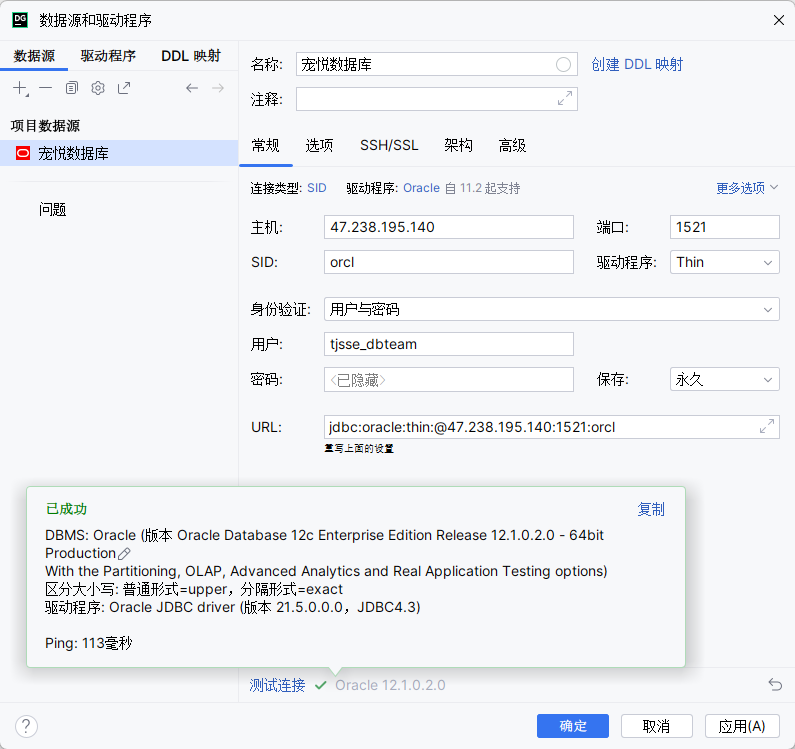
\includegraphics[width=\textwidth]{figures/ConnectViaDataGrip.png}
	\caption{通过JetBrains DataGrip连接数据库}
	\label{fig:ConnectViaDataGrip}
\end{figure}

\begin{itemize}
	\item \textbf{主机}:47.238.195.140
	\item \textbf{端口}:1521
	\item \textbf{SID}:orcl
	\item \textbf{驱动程序}:Thin
	\item \textbf{身份验证}:用户与密码
	\item \textbf{用户}:tjsse\_dbteam
	\item \textbf{密码}:tjsse2024
	\item \textbf{保存}:永久
	\item \textbf{URL}:jdbc:oracle:thin:@47.238.195.140:1521:orcl
\end{itemize}